% This LaTeX was auto-generated from MATLAB code.
% To make changes, update the MATLAB code and export to LaTeX again.

\documentclass{article}

\usepackage[utf8]{inputenc}
\usepackage[T1]{fontenc}
\usepackage{lmodern}
\usepackage{graphicx}
\usepackage{color}
\usepackage{hyperref}
\usepackage{amsmath}
\usepackage{amsfonts}
\usepackage{epstopdf}
\usepackage[table]{xcolor}
\usepackage{matlab}

\sloppy
\epstopdfsetup{outdir=./}
\graphicspath{ {./Homework3_shaobow_images/} }

\begin{document}

\begin{par}
\begin{flushleft}
Problem 1
\end{flushleft}
\end{par}

\begin{matlabcode}
clear; clc  
\end{matlabcode}

\begin{par}
\begin{flushleft}
(a)
\end{flushleft}
\end{par}

\begin{par}
\begin{flushleft}
The delayed system with RHP zero:
\end{flushleft}
\end{par}

\begin{matlabcode}
s = tf('s');
T_d = 5*10^-3;
G = (-s+3)/(s+2)/(s+1000)*exp(-T_d*s);
\end{matlabcode}

\begin{par}
\begin{flushleft}
Use inverse-based loop shaping to design controller. The basic loop shape of $\frac{s+a\omega_c }{s^2 (s+b\omega_c )}$ will create at least -90 deg's phase lag at crossover frequency. In order to have 40 deg's PM, the phase lag caused by time delay and RHP zero should be at most -50 deg.
\end{flushleft}
\end{par}

\begin{par}
\begin{flushleft}
Therefore, the crossover frequency has a upper bound:
\end{flushleft}
\end{par}

\begin{par}
$$-2\tan^{-1} (\frac{\omega_c }{3})>-50\deg \Rightarrow \omega_c <1.4rad/s$$
\end{par}

\begin{par}
\begin{flushleft}
Assume $\left\lbrace \begin{array}{c}
a=\frac{1}{\alpha }\\
b=\alpha 
\end{array}\right.$, and tune $\omega_c \;$and $\alpha$ to meet specifications.
\end{flushleft}
\end{par}

\begin{matlabcode}
w_c = 1.4;  % start with theoretical UB
while true
    alpha = 10^4;  % start with large enough alpha
    alpha_left = 0;
    alpha_right = alpha;
    a = 1/alpha;
    b = alpha;
    L = (s+a*w_c)/(s+b*w_c)/s^2*(-s+3)/(s+3)*exp(-T_d*s);
    [mag,~] = bode(L,w_c);
    L = 1/mag*L;
    [GM,PM] = margin(L);
    if db(GM)<6 || PM<40  % decrease wc if large alpha can't meet
        w_c = w_c-0.01;
    else
        while true  % bisect alpha 
            alpha_old = alpha;
            alpha = (alpha_left+alpha_right)/2;
            a = 1/alpha;
            b = alpha;
            L = (s+a*w_c)/(s+b*w_c)/s^2*(-s+3)/(s+3)*exp(-T_d*s);
            [mag,~] = bode(L,w_c);
            L = 1/mag*L;
            [GM,PM] = margin(L);
            if abs(alpha-alpha_old) < 1e-6
                break
            elseif abs(db(GM))>=6 && PM>=40
                alpha_right = alpha;
            else
                alpha_left = alpha;
            end
        end
        break
    end
end
\end{matlabcode}

\begin{par}
\begin{flushleft}
The maximized crossover frequency:
\end{flushleft}
\end{par}

\begin{matlabcode}
w_c
\end{matlabcode}
\begin{matlaboutput}
w_c = 1.3800
\end{matlaboutput}

\begin{par}
\begin{flushleft}
The designed controller:
\end{flushleft}
\end{par}

\begin{matlabcode}
[a*w_c;b*w_c]
\end{matlabcode}
\begin{matlaboutput}
ans = 2x1    
    0.0024
  791.4777

\end{matlaboutput}

\begin{par}
$$K=\frac{(s+a\omega_c )(s+2)(s+1000)}{s^2 (s+b\omega_c )(s+3)}=\frac{(s+0.0024)(s+2)(s+1000)}{s^2 (s+791.5)(s+3)}$$
\end{par}

\begin{par}
\begin{flushleft}
The final achieved loop shape and stability margin:
\end{flushleft}
\end{par}

\begin{matlabcode}
bode(L,[a*w_c,b*w_c],'o')
hold on
margin(L);
hold off
\end{matlabcode}
\begin{center}
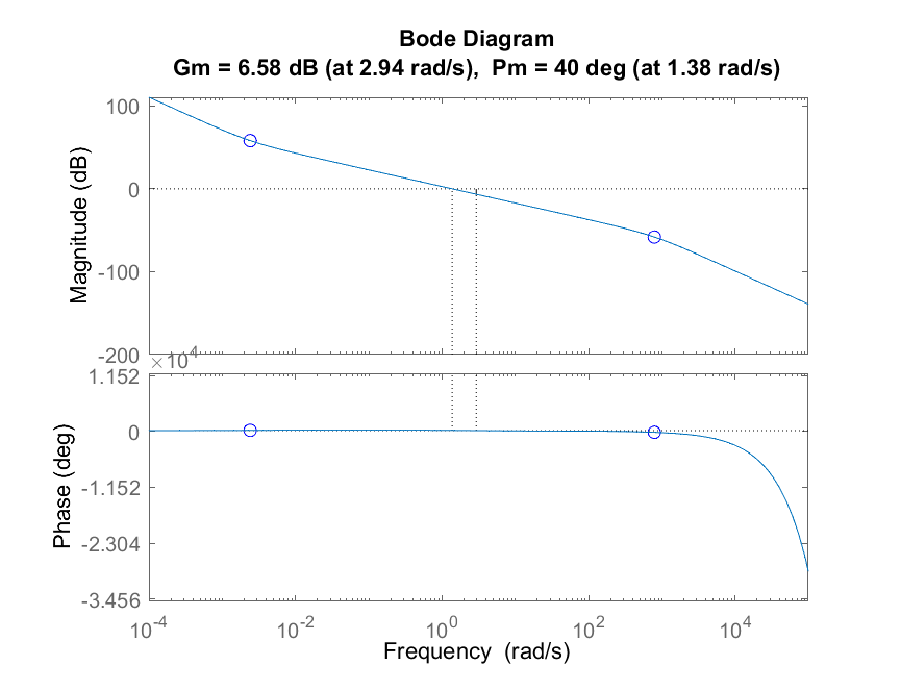
\includegraphics[width=\maxwidth{56.196688409433015em}]{figure_0.eps}
\end{center}

\begin{par}
\begin{flushleft}
Sensitivity function:
\end{flushleft}
\end{par}

\begin{matlabcode}
S = 1/(1+L);
bodemag(S);
\end{matlabcode}
\begin{center}
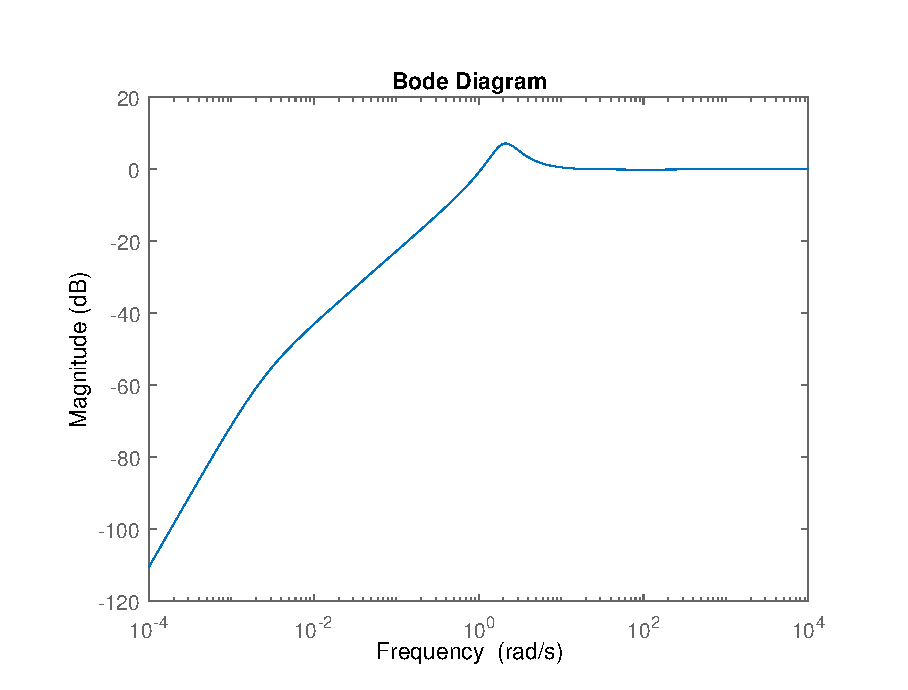
\includegraphics[width=\maxwidth{56.196688409433015em}]{figure_1.eps}
\end{center}

\begin{par}
\begin{flushleft}
(b)
\end{flushleft}
\end{par}

\begin{par}
\begin{flushleft}
For a unstable system without time delay:
\end{flushleft}
\end{par}

\begin{matlabcode}
clear;clc
s = tf('s');
G = (s+5)/(-s+1)/(s+1000);
\end{matlabcode}

\begin{par}
\begin{flushleft}
Use Loopsyn to design the controller, and start with a relatively high frequency of 2 kHz:
\end{flushleft}
\end{par}

\begin{matlabcode}
w_c = 2000;
G_d = w_c/s;
[K,CL,GAM] = loopsyn(G,G_d);
\end{matlabcode}

\begin{par}
\begin{flushleft}
The designed open-loop shape w.r.t desired upper bound and lower bound:
\end{flushleft}
\end{par}

\begin{matlabcode}
bodemag(G_d/GAM,G*K,G_d*GAM);
\end{matlabcode}
\begin{center}
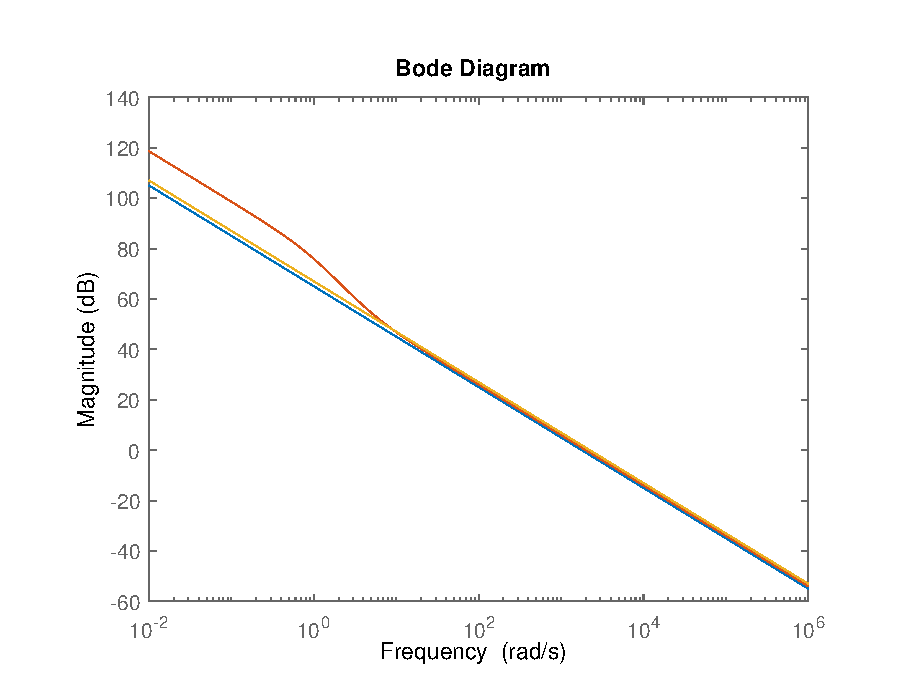
\includegraphics[width=\maxwidth{56.196688409433015em}]{figure_2.eps}
\end{center}

\begin{par}
\begin{flushleft}
Check margins to see if specs are met:
\end{flushleft}
\end{par}

\begin{matlabcode}
L = G*K;
margin(L);
\end{matlabcode}
\begin{center}
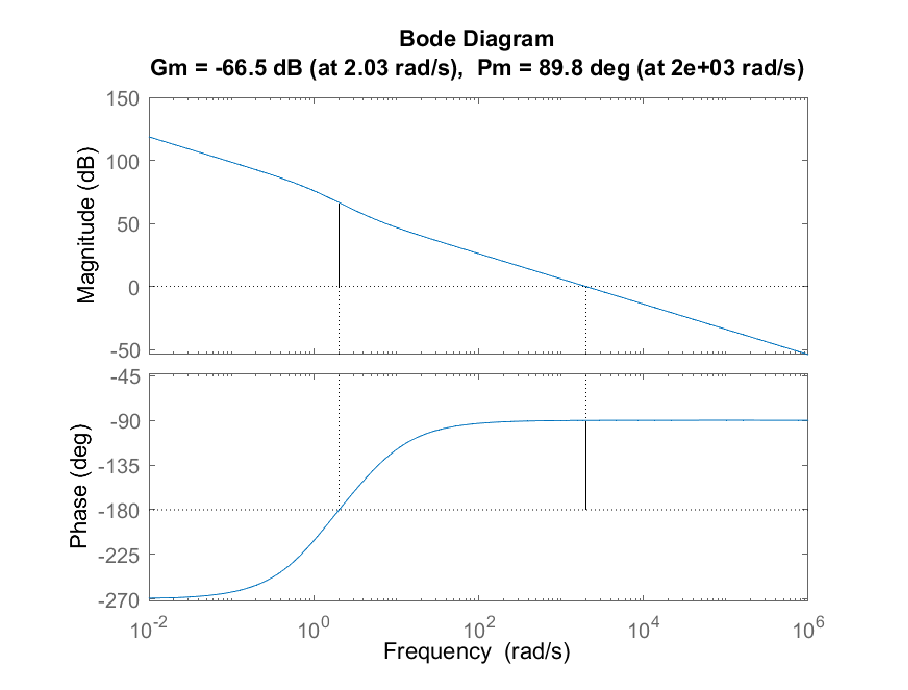
\includegraphics[width=\maxwidth{56.196688409433015em}]{figure_3.eps}
\end{center}

\begin{par}
\begin{flushleft}
Since the plant is unstable, the absolute value of GM satisfies the specs.
\end{flushleft}
\end{par}

\begin{matlabcode}
isStable = isstable(feedback(L,1))
\end{matlabcode}
\begin{matlaboutput}
isStable = 
   1

\end{matlaboutput}

\begin{par}
\begin{flushleft}
As demonstrated, the closed-loop system is stable.
\end{flushleft}
\end{par}


\begin{par}
\begin{flushleft}
Problem 2
\end{flushleft}
\end{par}

\begin{par}
\begin{flushleft}
(a)
\end{flushleft}
\end{par}

\begin{matlabcode}
clear;clc
\end{matlabcode}

\begin{par}
\begin{flushleft}
Input the HDD model:
\end{flushleft}
\end{par}

\begin{matlabcode}
HDDModel;
s = tf('s');
\end{matlabcode}

\begin{par}
\begin{flushleft}
The desired performance weight shape:
\end{flushleft}
\end{par}

\begin{matlabcode}
M = 2;  % 6dB
A = 0.001;  % -60dB
BWp = 3*10^3*2*pi;  % 3kHz
Wp_1 = makeweight(1/A,BWp,1/M);
Wp_2 = (s/sqrt(M)+BWp)^2/(s+BWp*sqrt(A))^2;
\end{matlabcode}

\begin{par}
\begin{flushleft}
Design the controller with performance sensitivity weights:
\end{flushleft}
\end{par}

\begin{matlabcode}
[K_1,CL_1,GAM_1] = mixsyn(P,Wp_1,[],[]);
[K_2,CL_2,GAM_2] = mixsyn(P,Wp_2,[],[]);
\end{matlabcode}

\begin{par}
\begin{flushleft}
The sensitivity function and desired sensitivity function using first-order method:
\end{flushleft}
\end{par}

\begin{matlabcode}
S_1 = 1/(1+P*K_1);
T_1 = 1-S_1;
bodemag(1/Wp_1,S_1);
legend('1/Wp1','S1','location','southeast')
\end{matlabcode}
\begin{center}
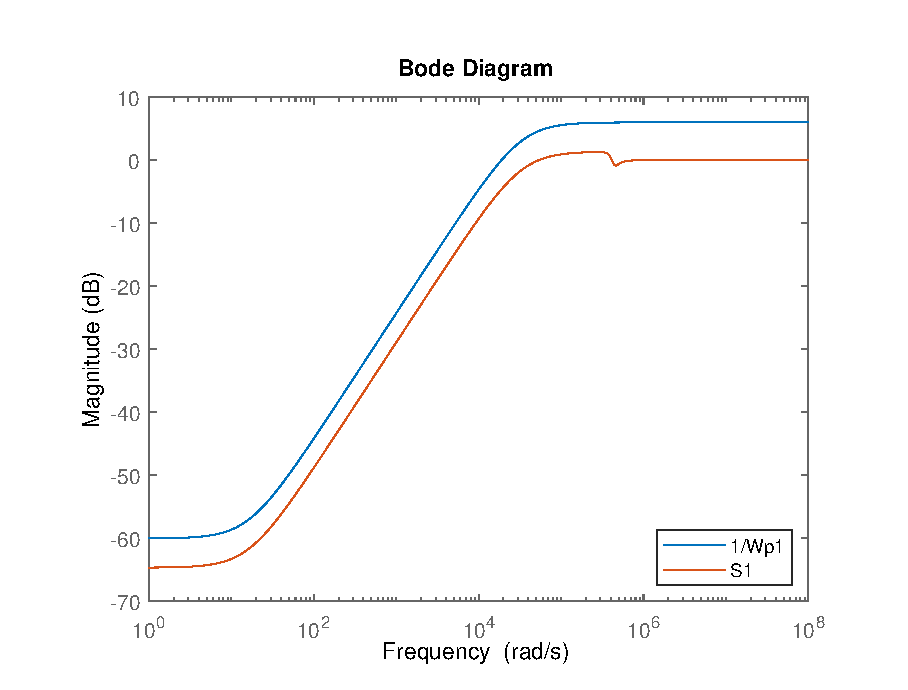
\includegraphics[width=\maxwidth{56.196688409433015em}]{figure_4.eps}
\end{center}

\begin{par}
\begin{flushleft}
The sensitivity function and desired sensitivity function using second-order method:
\end{flushleft}
\end{par}

\begin{matlabcode}
S_2 = 1/(1+P*K_2);
T_2 = 1-S_2;
bodemag(1/Wp_2,S_2);
legend('1/Wp2','S2','location','southeast')
\end{matlabcode}
\begin{center}
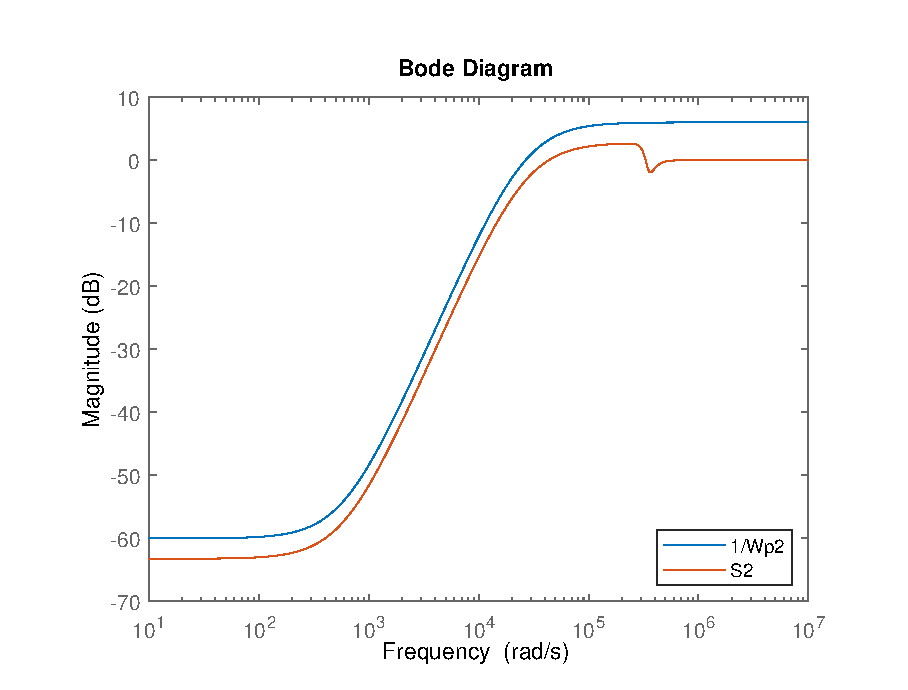
\includegraphics[width=\maxwidth{56.196688409433015em}]{figure_5.eps}
\end{center}

\begin{par}
\begin{flushleft}
Step response of both first-order and second-order methods design:
\end{flushleft}
\end{par}

\begin{matlabcode}
step(T_1,T_2);
legend('T1','T2','location','southeast')
\end{matlabcode}
\begin{center}
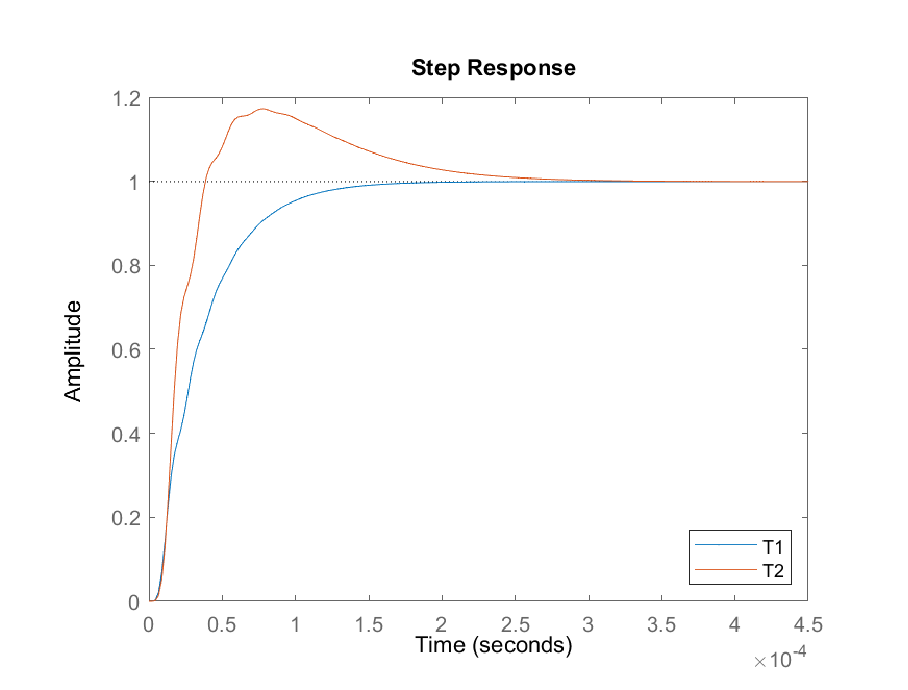
\includegraphics[width=\maxwidth{56.196688409433015em}]{figure_6.eps}
\end{center}

\begin{par}
\begin{flushleft}
The sensitivity crossing frequency will have a maximum boundary. 
\end{flushleft}
\end{par}

\begin{par}
\begin{flushleft}
(b)
\end{flushleft}
\end{par}

\begin{par}
\begin{flushleft}
The desired complementary sensitivity weight (already tuned to meet GAM\_pt \textless{} 1):
\end{flushleft}
\end{par}

\begin{matlabcode}
Mt = sqrt(2);  % 3dB
At = 0.5;
BWt = 10^4*2*pi;  % 10kHz
Wt = makeweight(1/Mt,BWt,1/At);  % 20dB/dec
\end{matlabcode}

\begin{par}
\begin{flushleft}
Design the controller with performance sensitivity and complementary sensitivity weights:
\end{flushleft}
\end{par}

\begin{matlabcode}
[K_pt,CL_pt,GAM_pt] = mixsyn(P,Wp_2,[],Wt);  % order matters
\end{matlabcode}

\begin{par}
\begin{flushleft}
Check that $\frac{1}{W_P }+\frac{1}{W_T }\ge 1$: 
\end{flushleft}
\end{par}

\begin{matlabcode}
weightbound = 1/norm(1/(1/Wp_2+1/Wt), 'inf')
\end{matlabcode}
\begin{matlaboutput}
weightbound = 1.1499
\end{matlaboutput}

\begin{par}
\begin{flushleft}
The sensitivity function and sensitivity weight function:
\end{flushleft}
\end{par}

\begin{matlabcode}
S_pt = 1/(1+P*K_pt);
bodemag(1/Wp_2,S_pt);
legend('1/Wp','Spt','location','southeast')
\end{matlabcode}
\begin{center}
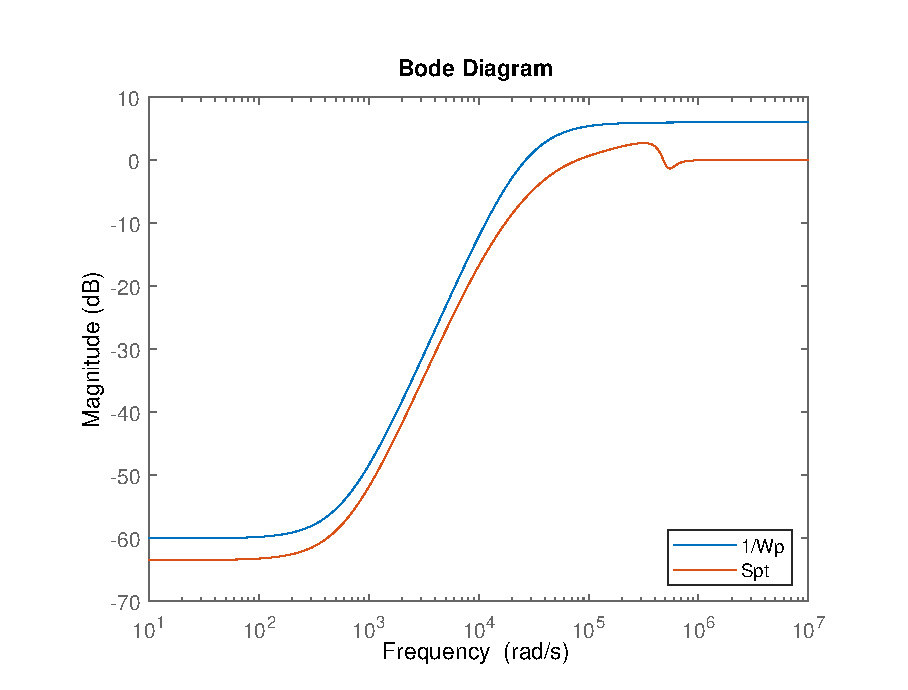
\includegraphics[width=\maxwidth{56.196688409433015em}]{figure_7.eps}
\end{center}

\begin{par}
\begin{flushleft}
The complementary sensitivity function and complementary sensitivity weight function:
\end{flushleft}
\end{par}

\begin{matlabcode}
T_pt = 1-S_pt;
bodemag(1/Wt,T_pt);
legend('1/W_t','Tpt','location','southeast')
\end{matlabcode}
\begin{center}
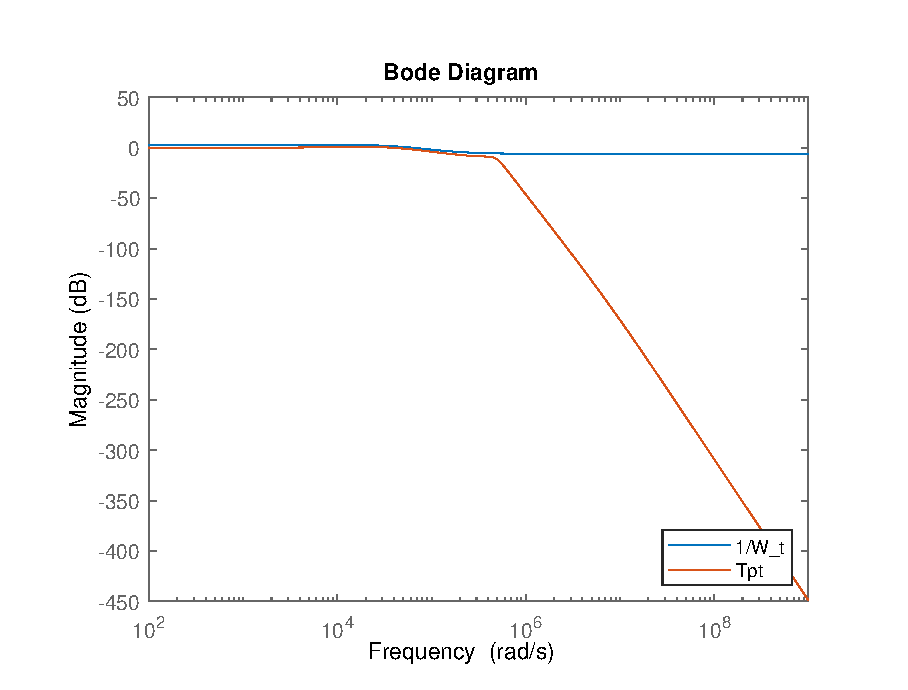
\includegraphics[width=\maxwidth{56.196688409433015em}]{figure_8.eps}
\end{center}

\begin{par}
\begin{flushleft}
(c) 
\end{flushleft}
\end{par}

\begin{par}
\begin{flushleft}
Include control weight:
\end{flushleft}
\end{par}

\begin{matlabcode}
Wu = 1/100;
\end{matlabcode}

\begin{par}
\begin{flushleft}
Use iteration method to achieve GAM \textless{} 1:
\end{flushleft}
\end{par}

\begin{matlabcode}
BW_right = 10^8*2*pi; 
BW_left = 0;
Wp = 0;
Wt = 0;
GAM_ms = 0;
while true
    GAM_old = GAM_ms;
    BW = (BW_left+BW_right)/2;
    Wp = (makeweight(sqrt(1/A),BW,sqrt(1/M)))^2;
    Wt = makeweight(1/Mt,5*BW,1/At);
    [K_ms,CL_ms,GAM_ms] = mixsyn(P,Wp,Wu,Wt);
    if abs(GAM_ms-GAM_old)<1e-6
        break
    elseif GAM_ms<1
        BW_left = BW;  
    else
        BW_right = BW;
    end
end
\end{matlabcode}

\begin{par}
\begin{flushleft}
The system sensitivity function and complementary sensitivity function:
\end{flushleft}
\end{par}

\begin{matlabcode}
L_ms = P*K_ms;
S_ms = 1/(1+L_ms);
T_ms = 1-S_ms;
\end{matlabcode}

\begin{par}
\begin{flushleft}
The sensitivity function and sensitivity weight function:
\end{flushleft}
\end{par}

\begin{matlabcode}
bodemag(1/Wp,S_ms);
legend('1/Wp','Sms','location','southeast')
\end{matlabcode}
\begin{center}
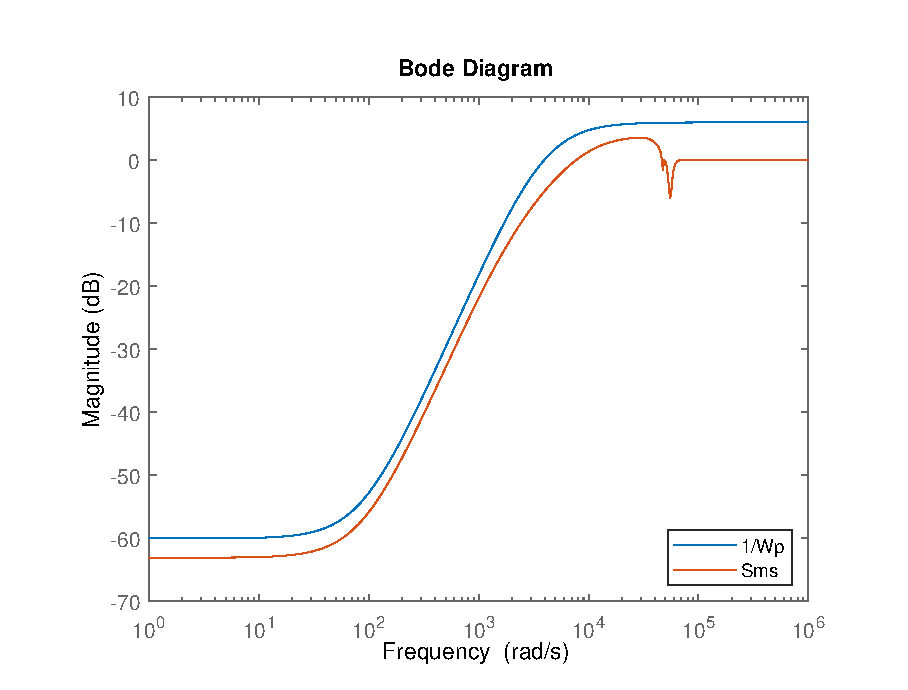
\includegraphics[width=\maxwidth{56.196688409433015em}]{figure_9.eps}
\end{center}

\begin{par}
\begin{flushleft}
The control function and control weight function:
\end{flushleft}
\end{par}

\begin{matlabcode}
bodemag(tf(1/Wu,1),K_ms*S_ms);
legend('1/Wu','Sms','location','southeast')
\end{matlabcode}
\begin{center}
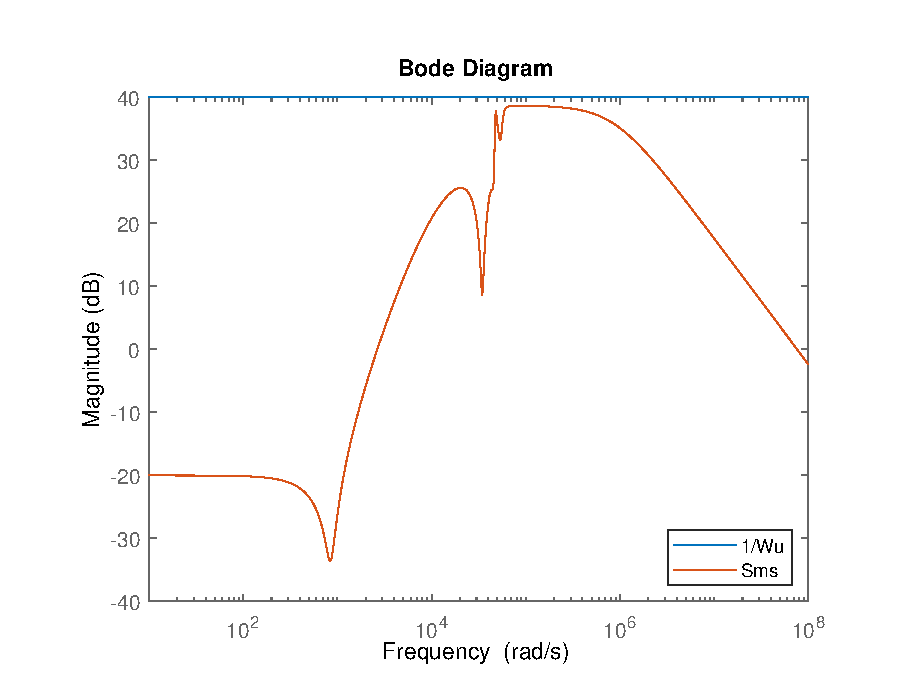
\includegraphics[width=\maxwidth{56.196688409433015em}]{figure_10.eps}
\end{center}

\begin{par}
\begin{flushleft}
The complementary sensitivity function and complementary sensitivity weight function:
\end{flushleft}
\end{par}

\begin{matlabcode}
bodemag(1/Wt,T_ms);
legend('1/Wt','Sms','location','southeast')
\end{matlabcode}
\begin{center}
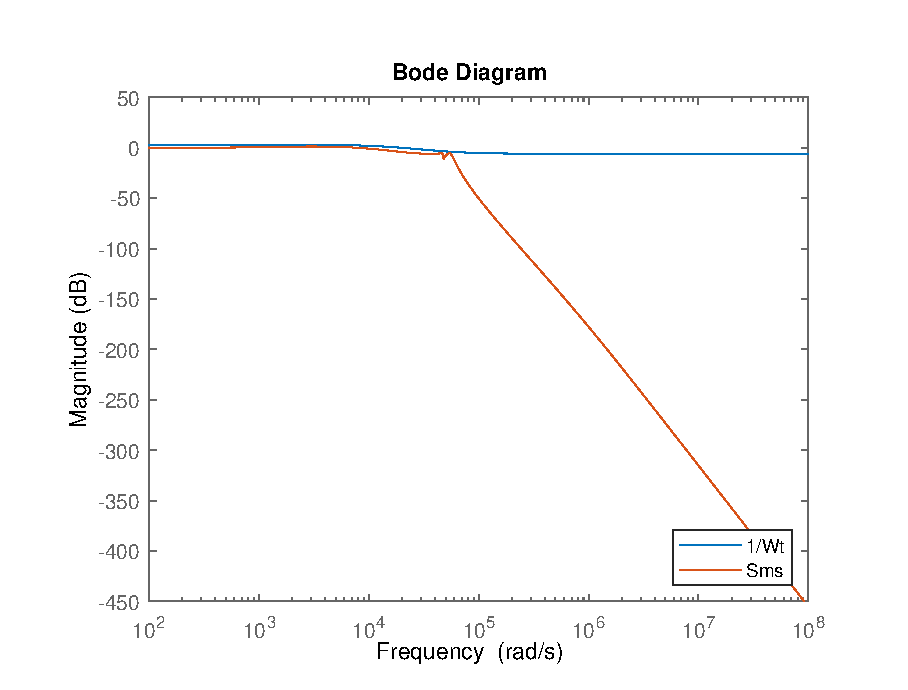
\includegraphics[width=\maxwidth{56.196688409433015em}]{figure_11.eps}
\end{center}

\begin{par}
\begin{flushleft}
The final $H_{\infty }$ norm:
\end{flushleft}
\end{par}

\begin{matlabcode}
N = [Wp*S_ms;Wu*K_ms*S_ms;Wt*T_ms];
H_inf_N = norm(N,'inf')
\end{matlabcode}
\begin{matlaboutput}
H_inf_N = 3.1614
\end{matlaboutput}
\begin{matlabcode}
H_inf_CL = norm(CL_ms,'inf')
\end{matlabcode}
\begin{matlaboutput}
H_inf_CL = 0.9966
\end{matlaboutput}
\begin{matlabcode}
% H_inf_p = norm(Wp*S_ms,'inf')
% H_inf_u = norm(Wu*K_ms*S_ms,'inf')
% H_inf_t = norm(Wt*T_ms,'inf')
\end{matlabcode}

\begin{par}
\begin{flushleft}
No idea why they have different values...
\end{flushleft}
\end{par}

\begin{par}
\begin{flushleft}
But the closed-loop system is stable with the designed controller:
\end{flushleft}
\end{par}

\begin{matlabcode}
isStable = isstable(feedback(K_ms*P,1))
\end{matlabcode}
\begin{matlaboutput}
isStable = 
   1

\end{matlaboutput}


\begin{par}
\begin{flushleft}
Problem 3
\end{flushleft}
\end{par}

\begin{matlabcode}
clear; clc
\end{matlabcode}

\begin{par}
\begin{flushleft}
(a)
\end{flushleft}
\end{par}

\begin{par}
\begin{flushleft}
Input dual-stage HDD model:
\end{flushleft}
\end{par}

\begin{matlabcode}
HDDModel_DS;
s = tf('s');
\end{matlabcode}

\begin{par}
\begin{flushleft}
Stack seperate TFs to get DISO system TF matrix:
\end{flushleft}
\end{par}

\begin{par}
$$y=\left\lbrack \begin{array}{cc}
VCM & PZT
\end{array}\right\rbrack \left\lbrack \begin{array}{c}
u_{VCM} \\
u_{PZT} 
\end{array}\right\rbrack$$
\end{par}

\begin{matlabcode}
G = [VCM,PZT];
\end{matlabcode}

\begin{par}
\begin{flushleft}
DISO system Bode plots:
\end{flushleft}
\end{par}

\begin{matlabcode}
bode(G);
\end{matlabcode}
\begin{center}
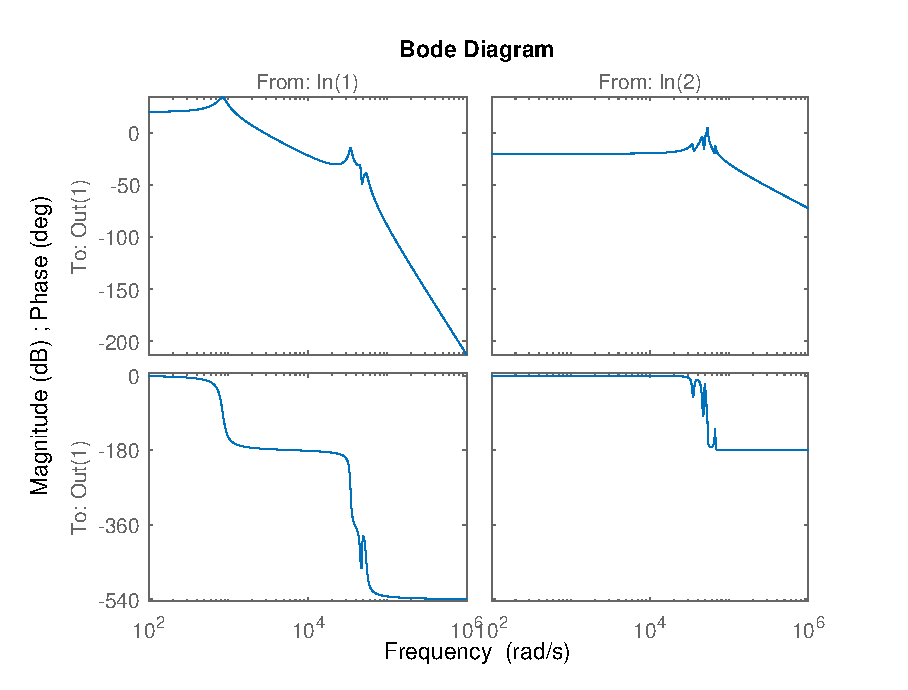
\includegraphics[width=\maxwidth{56.196688409433015em}]{figure_12.eps}
\end{center}

\begin{par}
\begin{flushleft}
(b)
\end{flushleft}
\end{par}

\begin{par}
\begin{flushleft}
Actuator saturations:
\end{flushleft}
\end{par}

\begin{matlabcode}
Wu_vcm = 1/100;
Wu_pzt = 1/10;
\end{matlabcode}

\begin{par}
\begin{flushleft}
Same specs from previous question:
\end{flushleft}
\end{par}

\begin{matlabcode}
M = 2;  % 6dB
A = 0.001;  % -60dB
Mt = sqrt(2);  % 3dB
At = 0.5;
\end{matlabcode}

\begin{par}
\begin{flushleft}
Use iteration method to achieve GAM \textless{} 1:
\end{flushleft}
\end{par}

\begin{matlabcode}
BW_right = 10^8*2*pi; 
BW_left = 0;
Wp = 0;
Wt = 0;
Wu = [Wu_vcm,0;0,Wu_pzt];
GAM_ms = 0;
while true
    GAM_old = GAM_ms;
    BW = (BW_left+BW_right)/2;
    Wp = (makeweight(sqrt(1/A),BW,sqrt(1/M)))^2;
    Wt = makeweight(1/Mt,5*BW,1/At);
    [K_ms,CL_ms,GAM_ms] = mixsyn(G,Wp,Wu,Wt);
    if abs(GAM_ms-GAM_old)<1e-4
        break
    elseif GAM_ms<1
        BW_left = BW;  
    else
        BW_right = BW;
    end
end
\end{matlabcode}

\begin{par}
\begin{flushleft}
The system sensitivity function and complementary sensitivity function:
\end{flushleft}
\end{par}

\begin{matlabcode}
L_ms = G*K_ms;
S_ms = eye/(eye+L_ms);
T_ms = eye-S_ms;
\end{matlabcode}

\begin{par}
\begin{flushleft}
The sensitivity function and sensitivity weight function:
\end{flushleft}
\end{par}

\begin{matlabcode}
bodemag(1/Wp,S_ms);
legend('1/Wp','Sms','location','southeast')
\end{matlabcode}
\begin{center}
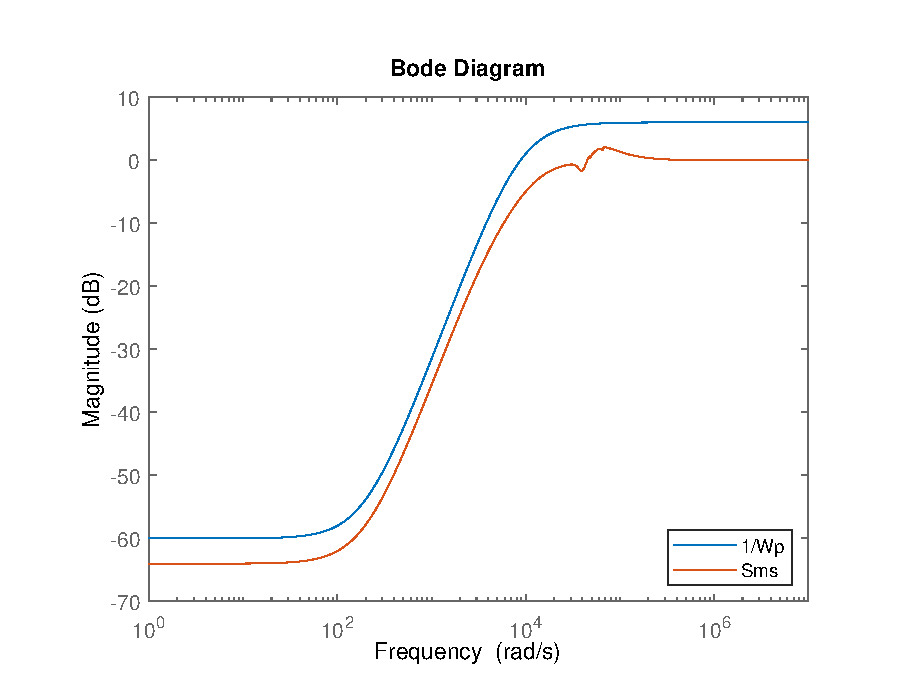
\includegraphics[width=\maxwidth{56.196688409433015em}]{figure_13.eps}
\end{center}

\begin{par}
\begin{flushleft}
The mags of $W_U KS$ are below 0 dB:
\end{flushleft}
\end{par}

\begin{matlabcode}
bodemag(Wu*K_ms*S_ms,[tf(1,1);tf(1,1)]);
\end{matlabcode}
\begin{center}
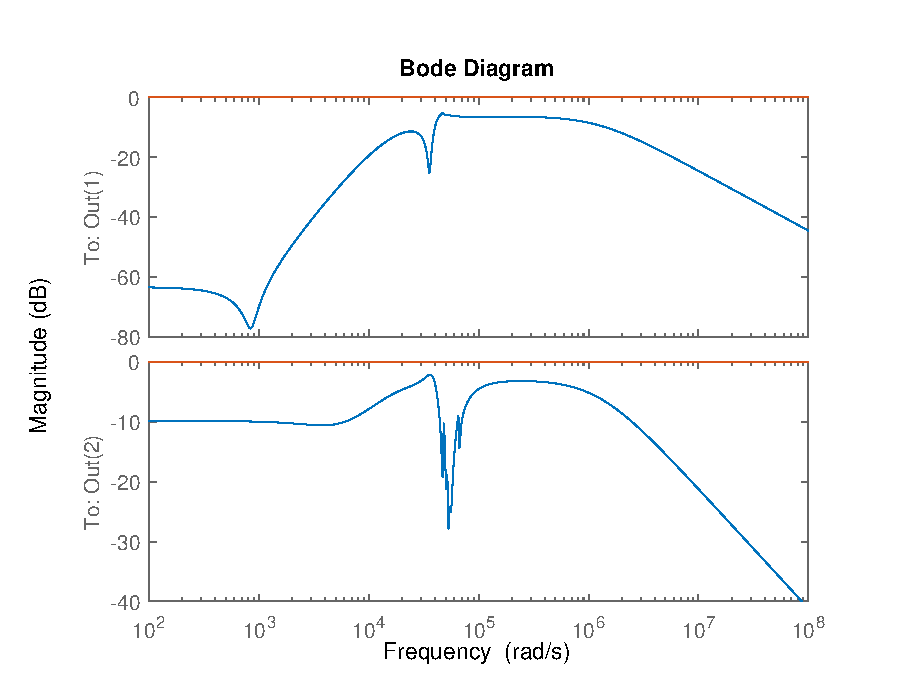
\includegraphics[width=\maxwidth{56.196688409433015em}]{figure_14.eps}
\end{center}

\end{document}
